\documentclass{beamer}
\usetheme[white]{Wisconsin}
\usepackage{longtable}
\usepackage{listings}
\usepackage{color}
%% The amssymb package provides various useful mathematical symbols
\usepackage{amssymb}
%% The amsthm package provides extended theorem environments
\usepackage{amsthm} \usepackage{amsmath}
%% \usepackage{eqnarray}
\usepackage[mathcal]{euscript} \usepackage{color}
\usepackage{textcomp}
\usepackage{algorithm,algorithmic}
\usepackage[retainorgcmds]{IEEEtrantools}
\usepackage[absolute,overlay]{textpos}
\usepackage{graphicx}
  \setlength{\TPHorizModule}{1mm}
  \setlength{\TPVertModule}{1mm}
\definecolor{listinggray}{gray}{0.9}
\definecolor{lbcolor}{rgb}{0.9,0.9,0.9}
\lstset{
  backgroundcolor=\color{lbcolor},
  tabsize=4,
  rulecolor=,
  language=c++,
  basicstyle=\scriptsize,
  upquote=true,
  aboveskip={1.5\baselineskip},
  columns=fixed,
  showstringspaces=false,
  extendedchars=true,
  breaklines=true,
  prebreak =
  \raisebox{0ex}[0ex][0ex]{\ensuremath{\hookleftarrow}},
  frame=single,
  showtabs=false,
  showspaces=false,
  showstringspaces=false,
  identifierstyle=\ttfamily,
  keywordstyle=\color[rgb]{0,0,1},
  commentstyle=\color[rgb]{0.133,0.545,0.133},
  stringstyle=\color[rgb]{0.627,0.126,0.941},
}

%% colors
\setbeamercolor{boxheadcolor}{fg=white,bg=UWRed}
\setbeamercolor{boxbodycolor}{fg=black,bg=white}

%%----------------------------------------------------------------------------%%
\author{Luke J. Kersting
    \\ NEEP
    \\ University of Wisconsin - Madison
    \\ FRENSIE Meeting
}

\date{\today}
\title{Moment Preserving Monte Carlo Electron Transport}
\begin{document}
\maketitle

%%----------------------------------------------------------------------------%%
\begin{frame}{Outline}

    \begin{itemize}
      \item Monte Carlo Electron Transport
      \item Analog Transport Method
      \item Condensed History Method
      \item Moment Preserving Method
      \item Evaluated Electron Data Library
      \item Implementation
      \item Future Work
    \end{itemize}

\end{frame}

%%----------------------------------------------------------------------------%%
\begin{frame}{The Monte Carlo Method}

    \begin{itemize}
      \item A stochastic method using random numbers
      \item Samples a population of events based on a set of probabilities
      \item Enough event can accurately represent a distribution
      \item Can produce a numerical answer for a complex system of processes
    \end{itemize}
    
    \begin{figure}
  \centering
  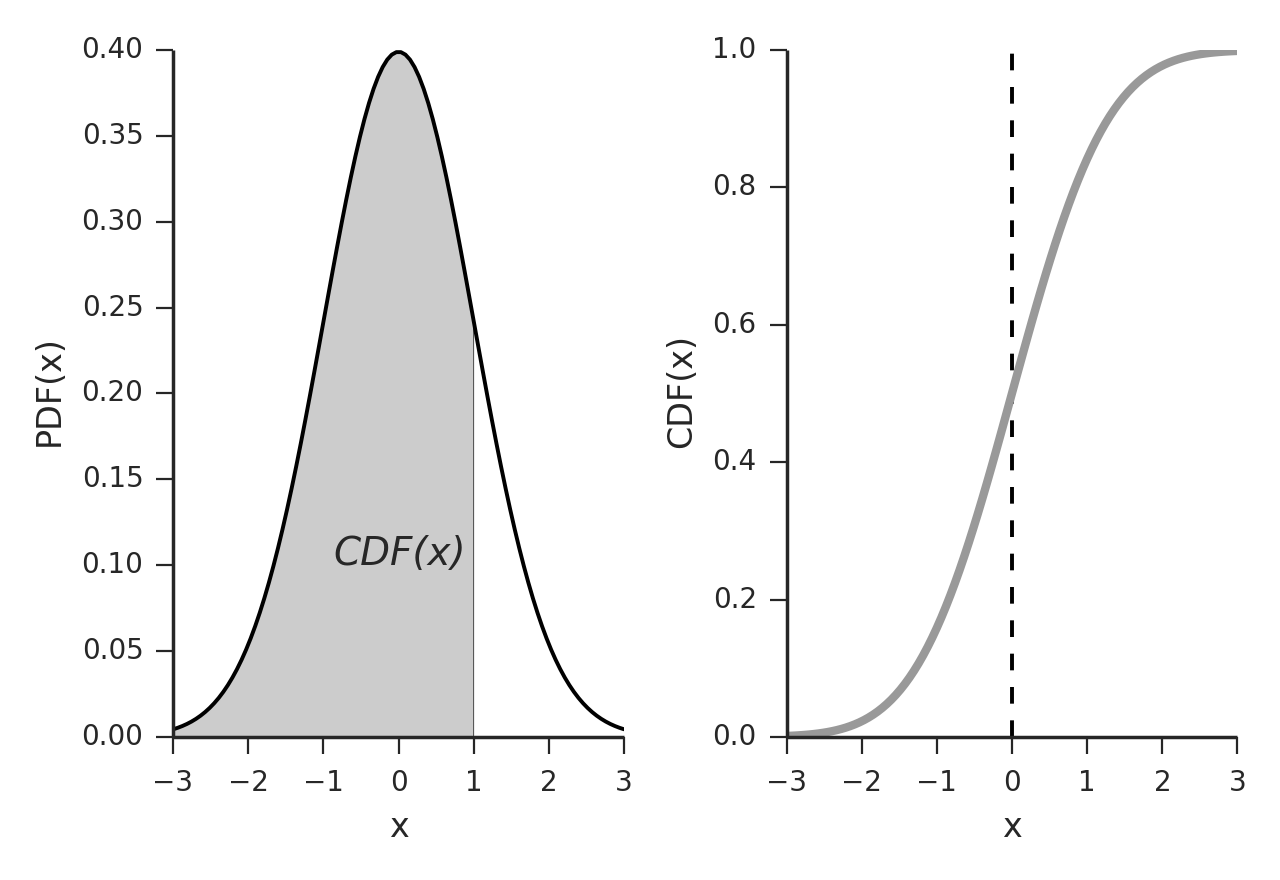
\includegraphics[width=70mm]{PDF_CDF.png}
  \caption{Example PDF and CDF of the value of x}
\end{figure}

\end{frame}

%%----------------------------------------------------------------------------%%
\begin{frame}{Monte Carlo Particle Transport}

 \begin{block}{Particles are taken through a random walk process}
 
 \begin{figure}
  \centering
  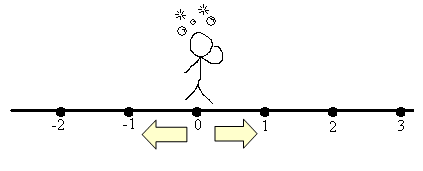
\includegraphics[width=50mm]{drunkchap.png}
\end{figure}

\end{block}

 \begin{block}{Individual events are sampled}
 
    \begin{itemize}
      \item Scattering
      \item Absorption
    \end{itemize}
    
\end{block}

 \begin{block}{For each event properties are randomly sampled}
    
     \begin{itemize}
      \item Energy
      \item Position
      \item Direction
      \item Secondary Particles
    \end{itemize}
\end{block}
 

\end{frame}

%%----------------------------------------------------------------------------%%
\begin{frame}{Monte Carlo Electron Transport}

  \begin{block}{Challenges}
    \begin{itemize}
      \item Electron charge increases scattering cross section
      \item Neutral Particles may scatter a couple dozen times over a distance
      \item Electrons may scatter 10,000 or more times over the same distance
      \item Purely analog transport is impractical at higher energies
      \item Approximations must be made to reduce computation costs
      \item Monte Carlo Electron development lags behind Neutron and Photon
    \end{itemize}
  \end{block}
    
  \begin{block}{Motivation}
    \begin{itemize}
      \item Electrons transport needed for precision dose and energy deposition calculations
      \item Secondary electrons in photon transport through high Z material
      \item Solid state physics
      \item Medical physics
    \end{itemize}    
  \end{block}  

\end{frame}

%%----------------------------------------------------------------------------%%
\begin{frame}{Condensed History Method}

  \begin{itemize}
    \item ``Condensed'' random walk method developed to speed up electron transport
    \item Electrons move a set step length that is many mean free paths 
    \item Multiple scattering theory sampled to get the outgoing direction
    \item The Continuous Slowing Down Approximation (CSDA) used to calculate energy loss
    \item Production of secondary particles are averaged
    \item Approximations don't hold below 1 keV
    \item Assumes infinite medium 
  \end{itemize}

\end{frame}

%%----------------------------------------------------------------------------%%
\begin{frame}{Condensed History Step}
  
\begin{figure}
  \centering
  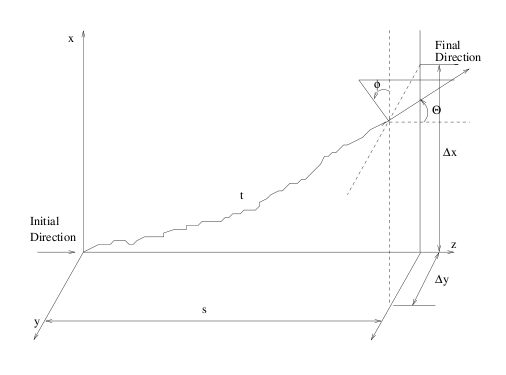
\includegraphics[width=90mm]{electron_step.png}
  \caption{Schematic of electron transport mechanics model in EGS. Where $s$ is the step length, $t$ the total distance travelled, $\Delta x$ and $\Delta y$ are the lateral displacements, $\Theta$ and $\phi$ are the final polar and azimuthal angles.}
\end{figure}

\end{frame}

%%----------------------------------------------------------------------------%%
\begin{frame}{Improving Condensed History}

\begin{block}{Improving Transport Mechanics}
  
  \begin{itemize}
    \item Random Hinge transport
    \item Modified Random Hinge transport
    \item Accurate Transport near boundaries
  \end{itemize}
  
\end{block}  

\begin{block}{Mixed Analog/Condensed Simulation}
  
  \begin{itemize}
    \item Hard events involving large angle scattering, secondary particles, and catastrophic interactions are analog
    \item Soft events involving small angle scattering are condensed
    \item Majority of electron cross section is due to soft elastic scattering
    \item Below 1 keV simulation becomes purely analog
  \end{itemize}
  
\end{block}  

\end{frame}

%%----------------------------------------------------------------------------%%

\begin{frame}{Moment Preserving Method (MP)}

  \begin{itemize}
\item Legendre moments of the cross section are preserved
  
  \begin{itemize}
    \item mfps are reduced, increasing efficiency
    \item Less forward peaked angular scattering distribution
    \item Accuracy can be maintained by preserving some of the low-order moments
  \end{itemize}

\item Simplified physics that reflect the analog process are used

\item Implementation simpler than Condensed History

\item Distribution is no longer continuous but discrete
  \end{itemize}

\end{frame}

%%----------------------------------------------------------------------------%%

\begin{frame}{Reduced Order Physics}

\begin{itemize}
 \item The Boltzmann collision operator is approximated using reduced order physics (ROP)
  
  \begin{itemize}
    \item Integral form maintained
    \item Keeps correct transport mechanics
    \item Allows single-event simulations
  \end{itemize}

 \item The analog cross section, $ \Sigma $, is replaced with a ROP cross section, $ \tilde{\Sigma} $
  \begin{itemize}
    \item  preserves a finite number of moments of the analog cross section
  \end{itemize}
  
\end{itemize}

	\begin{equation}
		\Sigma_n(E) = 2\pi \int_{-1}^{1}P_n(\mu_0)\Sigma(E,\mu_0)d\mu_0~.
	\end{equation}
	
	\begin{equation}
		\tilde{\Sigma}_n(E) = \Sigma_n(E)~.
	\end{equation}

\end{frame}

%%----------------------------------------------------------------------------%%

\begin{frame}{ROP Elastic Cross Section}

\begin{block}{MP Method Only}

\begin{equation}
	\tilde{\Sigma}_{el}(E,\mu_0) 
	= \frac{1}{2\pi}\sum_{m=1}^{M} \delta(\mu_0-\mu_m)\alpha_m
	 +\frac{1}{2\pi} \delta(\mu_0-\mu_{M+1})\alpha_{M+1}
\end{equation}
	
  \begin{itemize}
    \item Where  $\alpha_m$ and  $\mu_m$ are the weights and nodes of the Radau quadrature
    \item The $M+1$ node is fixed at $\mu_{M+1}=1$ (ie: no angular defection)
    \item The $M+1$ component can be removed from $\tilde{\Sigma}_{el}$
  \end{itemize}
  
  \begin{equation}
	\tilde{\Sigma}_{el}(E,\mu_0) 
	= \frac{1}{2\pi}\sum_{m=1}^{M} \delta(\mu_0-\mu_m)\alpha_m
\end{equation}

\end{block}

\end{frame}

%%----------------------------------------------------------------------------%%

\begin{frame}{ROP Elastic Cross Section}

\begin{block}{Hybrid Method}

  \begin{itemize}
    \item Below a cutoff, $\mu'$, analog transport is used
    
    	\begin{equation}
		\tilde{\Sigma}_{el}(E,\mu_0) 
		= \Sigma^S_{el}(E,\mu_0) + \frac{1}{2\pi}\sum_{m=1}^{M} \delta(\mu_0-\mu_m)\alpha_m(E)~.
		\label{eq:hybrid_elastic_dcs}
	\end{equation}
	
    \item Where $ \Sigma^S_{el}$ is the analog cross section for $\mu \in [-1,\mu']$
    \item Only discrete angles are used above  $\mu'$
  \end{itemize}

\end{block}

\begin{block}{Advantages}
  \begin{itemize}
    \item Discrete angles are only used for the highly forward peaked component
    \item Discrete artifacts are highly reduced
    \item Analog component increases accuracy and can easily be implemented
  \end{itemize}
\end{block}

\end{frame}

%%----------------------------------------------------------------------------%%
\begin{frame}{Single-Event Adjoint Electron Transport}

\begin{block}{Goals}
	\begin{itemize}
	\item Transform forward electron data to adjoint
	\item Use single-event EEDL data in transformation
	\item Output usable adjoint single-event electron cross-sections and PDF's
	\end{itemize}

\end{block}

\begin{block}{Four analog processes are represented}

  \begin{itemize}
    \item Atomic Excitation
    \item Electroionization
    \item Bremsstrahlung
    \item Elastic
  \end{itemize}

\end{block}

\end{frame}
%
%%----------------------------------------------------------------------------%%
\begin{frame}{Forward Transport}
\begin{block}{Time-Independent Boltzmann Equation}
\begin{multline}
  \Omega \nabla \phi(\boldsymbol r,E,\boldsymbol\Omega) + 
  \Sigma_t(\boldsymbol{r},E)\phi(\boldsymbol{r},E,\boldsymbol{\Omega}) = \\
  \int\int\Sigma_t(\boldsymbol{r},E')C(\boldsymbol{r},E'\rightarrow E,\boldsymbol{\Omega'}\rightarrow\boldsymbol{\Omega})\phi(\boldsymbol{r},E',\boldsymbol{\Omega'})dE'd\Omega' + 
  S(\boldsymbol{r},E,\boldsymbol{\Omega})
\end{multline}
\end{block}

\begin{block}{Collision Kernel}
\begin{multline}
C(\boldsymbol{r},E'\rightarrow E,\boldsymbol{\Omega'}\rightarrow\boldsymbol{\Omega}) = \\
\sum_A p_A(\boldsymbol{r},E') \sum_j p_{j,A}(E') c_{j,A}(E') f_{j,A}(E'\rightarrow E,\boldsymbol{\Omega'}\rightarrow\boldsymbol{\Omega})
\end{multline}

\begin{equation}
p_A(\boldsymbol{r},E') = \frac{\Sigma_A(\boldsymbol{r},E')}{\Sigma_t(\boldsymbol{r},E')}
~~~~~~~~~~~~~~~~~~
p_{j,A}(E') = \frac{\sigma_{j,A}(E')}{\sigma_A(E')} \nonumber
\end{equation}

\end{block}

\end{frame}

%%----------------------------------------------------------------------------%%
\begin{frame}{Adjoint Transport}

%\begin{block}{Time-Independent Boltzmann Equation}
%\begin{multline}
%  -\Omega \nabla \phi^{\dagger}(\boldsymbol r,E,\boldsymbol\Omega) + 
%  \Sigma_t(\boldsymbol{r},E)\phi^{\dagger}(\boldsymbol{r},E,\boldsymbol{\Omega}) = \\
%  \int\int\Sigma_t(\boldsymbol{r},E)C(\boldsymbol{r},E\rightarrow E',\boldsymbol{\Omega}\rightarrow\boldsymbol{\Omega})\phi^{\dagger}(\boldsymbol{r},E',\boldsymbol{\Omega})dE'd\Omega' + 
%  D(\boldsymbol{r},E,\boldsymbol{\Omega})
%\end{multline}
%\end{block}

\begin{block}{Adjoint Collision Kernel}
\begin{multline}
C^{\dagger}(\boldsymbol{r'},E'\rightarrow E,\boldsymbol{\Omega'}\rightarrow\boldsymbol{\Omega}) = \\
\sum_A p_A^{\dagger}(\boldsymbol{r'},E') \sum_j p^{\dagger}_{j,A}(E') \frac{\sigma_{j,A}(E)c_{j,A}(E)f_{j,A}(E\rightarrow E',\boldsymbol{\Omega}\rightarrow\boldsymbol{\Omega'})}{\sigma^{\dagger}_{j,A}(E')}
\end{multline}

\begin{equation}
\sigma^{\dagger}_{j,A}(E') = \int\sigma_{j,A}(E)c_{j,A}(E)f_{j,A}(E\rightarrow E')dE
\end{equation}

\begin{equation}
p^{\dagger}_A(\boldsymbol{r'},E') = \frac{\Sigma^{\dagger}_A(\boldsymbol{r'},E')}{\Sigma{\dagger}(\boldsymbol{r'},E')}
~~~~~~~~~~~~~~~~~~
p^{\dagger}_{j,A}(E') = \frac{\sigma^{\dagger}_{j,A}(E')}{\sigma^{\dagger}_A(E')} \nonumber
\end{equation}

\end{block}

\end{frame}

%%----------------------------------------------------------------------------%%
\begin{frame}{Adjoint Transport}

First the type of nuclide that the electron interacts with is sampled from:
\begin{equation}
p^{\dagger}_A(\boldsymbol{r'},E') = \frac{\Sigma^{\dagger}_A(\boldsymbol{r'},E')}{\Sigma{\dagger}(\boldsymbol{r'},E')}
\end{equation}

Then the reaction type is sampled from:
\begin{equation}
p^{\dagger}_{j,A}(E') = \frac{\sigma^{\dagger}_{j,A}(E')}{\sigma^{\dagger}_A(E')} \nonumber
\end{equation}

Finally, $E$ and $\Omega$ are sampled from:
\begin{equation}
f^{\dagger}_{j,A}(E'\rightarrow E,\boldsymbol{\Omega'}\rightarrow\boldsymbol{\Omega}) = 
\frac{\sigma_{j,A}(E)c_{j,A}(E)f_{j,A}(E\rightarrow E',\boldsymbol{\Omega}\rightarrow\boldsymbol{\Omega'})}{\sigma^{\dagger}_{j,A}(E')} \nonumber
\end{equation}

\end{frame}


%%----------------------------------------------------------------------------%%
\begin{frame}{Adjoint Cross-Sections}
Electrons reactions are not specifically dependent on the incoming and outgoing angle, 
but instead on $\mu$. Therefore the equations reduced to:
\begin{equation}
\sigma^{\dagger}(E') = \int\int\sigma(E)c(E)f(E \rightarrow E', \mu)dEd\mu
\end{equation}

\begin{equation}
f^{\dagger}(E' \rightarrow E, \mu) = \frac{\sigma(E)c(E)f(E \rightarrow E', \mu)}{\sigma^{\dagger}(E')}
\end{equation}

\begin{equation}
\sigma^{\dagger}(E' \rightarrow E, \mu) = \sigma(E \rightarrow E', \mu)
\end{equation}

\end{frame}

%%----------------------------------------------------------------------------%%
\begin{frame}{Elastic Scattering}
	\begin{itemize}
	\item Their is no energy loss ($ E = E'$)
	\item Adjoint and Forward transport will be exactly the same
	\end{itemize}
\begin{align}
\sigma^{\dagger}(E' \rightarrow E, \mu) = &\sigma(E \rightarrow E', \mu) = \nonumber \\
\sigma^{\dagger}(E, \mu) = &\sigma(E, \mu)
\end{align}

Therefore equations $(6)$ and $(7)$ reduce to:
\begin{equation}
\sigma^{\dagger}(E') = \sigma(E)
\end{equation}

\begin{equation}
f^{\dagger}(E, \mu) = f(E, \mu)
\end{equation}

\end{frame}

%%----------------------------------------------------------------------------%%
\begin{frame}{Elastic Scattering}

\begin{block}{Implementation in FRENSIE}
	\begin{itemize}
	\item Add the ability to take an adjoint particle to the forward class
	\item Add a scatter electron function       
	\end{itemize}
\end{block}

\end{frame}

%%----------------------------------------------------------------------------%%
\begin{frame}{Atomic Excitation}
	\begin{itemize}
	\item Their is no angular deflection
	\item Cross-sections are independent of angle
	\item Each incoming energy will scatter into a unique outgoing energy
	\item There is a one-to-one correspondence between the incoming and outgoing energy
	\end{itemize}

\begin{align}
\sigma^{\dagger}(E' \rightarrow E, \mu) = &\sigma(E \rightarrow E', \mu) = \nonumber \\
\sigma^{\dagger}(E') = &\sigma(E)
\end{align}

\begin{equation}
f^{\dagger}(E', \mu) = \frac{\sigma(E)f(E, \mu)}{\sigma^{\dagger}(E')} = f(E, \mu)
\end{equation}

\end{frame}

%%----------------------------------------------------------------------------%%
\begin{frame}{Atomic Excitation}

\begin{block}{Implementation in FRENSIE}
	\begin{itemize}
	\item Create energy dependent electron energy gain data tables
		\begin{itemize}
		\item Replace the incoming energy with the outgoing energy in the ACE energy loss tables
		\item Use interpolation to create a more uniform energy bin structure
		\end{itemize}
	
	\item Create Adjoint Atomic Excitation class similar to forward case
	\end{itemize}
\end{block}

\end{frame}

%%----------------------------------------------------------------------------%%
\begin{frame}{Bremsstrahlung}
	\begin{itemize}
	\item Angular deflection is assumed to be negligible
	\item Cross-sections are independent of angle
	\end{itemize}

\begin{align}
\sigma^{\dagger}(E' \rightarrow E, \mu) = & \sigma(E \rightarrow E', \mu) =\nonumber \\
\sigma^{\dagger}(E' \rightarrow E) = & \sigma(E \rightarrow E') = \sigma(E)f(E \rightarrow E')
\end{align}

\begin{equation}
\sigma^{\dagger}(E') = \int\sigma(E)f(E \rightarrow E')dE
\end{equation}

\begin{equation}
f^{\dagger}(E' \rightarrow E) = \frac{\sigma(E)f(E \rightarrow E')}{\sigma^{\dagger}(E')}
\end{equation}


\end{frame}

%%----------------------------------------------------------------------------%%
\begin{frame}{Bremsstrahlung}

\begin{block}{Implementation in FRENSIE}
	\begin{itemize}
	\item Create 2D electron energy gain pdf data tables
		\begin{itemize}
		\item Numerically integrate the cross section for a given energy loss over all incident energies
		\item Use interpolation to create a energy bin structure
		\item Create a pdf for each outgoing energy bin
		\end{itemize}
	
	\item Create new adjoint Bremsstrahlung class
	\end{itemize}
\end{block}

\end{frame}

%%----------------------------------------------------------------------------%%
\begin{frame}{Electroionization}
	\begin{itemize}
	\item A second electron is produced
	\item There is a unique angle for each $E \rightarrow E'$ pair
	\end{itemize}

\begin{equation}
p(E \rightarrow E', \mu) = f(E \rightarrow E')
\end{equation}

\begin{equation}
\sigma^{\dagger}(E') = \int\sigma(E)f(E \rightarrow E')dE
\end{equation}

\begin{equation}
f^{\dagger}(E'\rightarrow E, \mu) = \frac{\sigma(E)f(E \rightarrow E')}{\sigma^{\dagger}(E')} 
\end{equation}

\end{frame}

%%----------------------------------------------------------------------------%%
\begin{frame}{Braking Down the Adjoint Electroionization Cross-Section}
	\begin{itemize}
	\item The adjoint cross-section can be broken into two parts corresponding to the primary and secondary particle
	\item The primary particle has a energy range: ~~~~$E/2 \leq E' \leq E$
	\item The secondary particle has a energy range: ~$E_{min} \leq E' \leq E/2$
	\end{itemize}


\begin{align}
\sigma^{\dagger}(E') = &\sigma^{\dagger}_{prim}(E') + \sigma^{\dagger}_{sec}(E') \nonumber \\
= & \int\sigma(E) \Big( f_{prim}(E \rightarrow E') + f_{sec}(E \rightarrow E') \Big)dE
\end{align}

\end{frame}

%%----------------------------------------------------------------------------%%
\begin{frame}{Electroionization}

\begin{block}{Implementation in FRENSIE}
	\begin{itemize}
	\item Create 2D electron energy gain pdf data tables
		\begin{itemize}
		\item Numerically integrate the cross section for a given outgoing electron energy over all incident electron energies
		\item Use interpolation to create a energy bin structure
		\item Create a pdf for each knock-on energy bin
		\end{itemize}
	
	\item Create new adjoint Electroionization template class
	\end{itemize}
\end{block}

\end{frame}

%%----------------------------------------------------------------------------%%

\end{document}
